%!TEX root = paper_main.tex

\section{BLE Tracking Toolkit}
\label{sec:methodology}

In this section I present a high-level overview of the algorithm we use in this work to estimate the physical-layer properties of the BLE transmitters.
%
The mathematical details of the algorithm are beyond the scope of this dissertation, and therefore I only present the high level intuition to obtaining high-precision fingerprints from BLE beacons.

The hardware imperfections that lead to the fingerprint arise from the underlying manufacturing variations in BLE transmitter hardware.
%
These manufacturing variations lead to non-idealities in the received BLE beacon signals, which we can measure to derive the fingerprint.
%
In particular, most mobile devices feature an integrated single-chip WiFi+ BLE transmitter, which has a shared \iq frontend.
%
Therefore, the BLE transmissions are impacted by the same hardware imperfections as the WiFi transmitter.
%
For our work, we explore the following specific hardware imperfections:
\begin{enumerate}
    \item \textbf{CFO: } The Carrier Frequency Offset (CFO) is a shift in the carrier frequency from the ideal channel value. This arises due to the frequency error of the crystal oscillator that is used to generate the carrier signal that feeds into the mixer in the RF frontend.
    \item \textbf{\iq imperfections :} \iq Offset happens due either the leakage of the carrier signal onto the transmitter output due to non-idealities of the mixer hardware, or due to an DC offset on the baseband signals. \iq Imbalance is a deviation in amplitude and phase of transmitted signal, due to the mismatch between similar analog components on the in-phase and quadrature-phase paths.
    
\end{enumerate}
\begin{figure}
    \centering
    \captionsetup{justification=centering}
    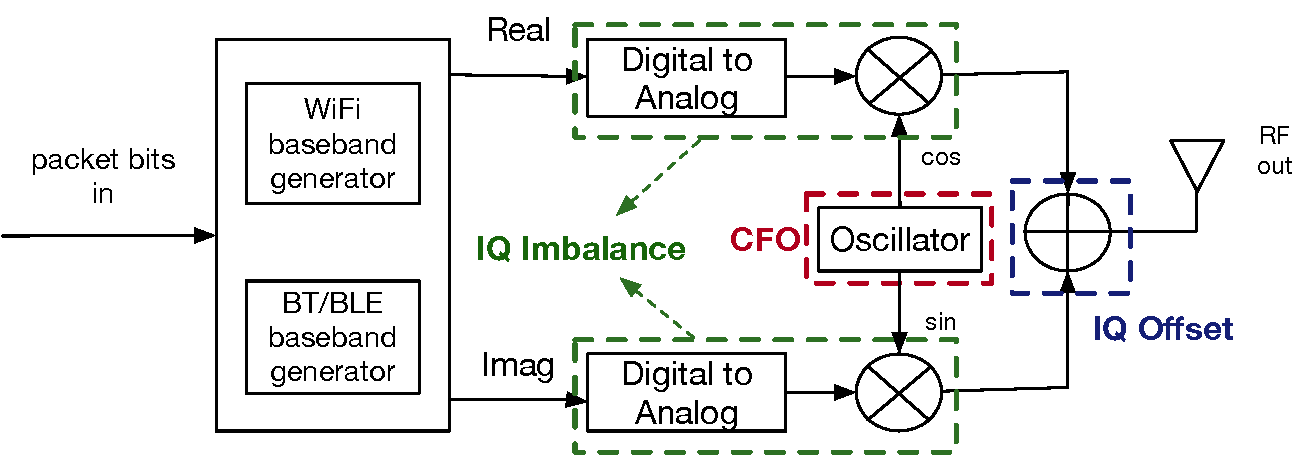
\includegraphics[width = 0.8\linewidth]{bletracking/plots/IQchain.pdf} 
    \caption{Architecture of WiFi/BLE combo chipsets}
    \label{fig:iq_arch}
\end{figure}
Figure~\ref{fig:iq_arch} shows the architecture of a typical BLE transmitter, and the sources of the imperfections described above.

Unfortunately, we can't reuse techniques from prior work on WiFi physical-layer fingerprinting to measure these properties precisely for Bluetooth LE. 
%
Prior techniques rely on the presence of a long known sequence or preamble as a reference to measure the signal distortions due to CFO and \iq imperfections accurately
%
BLE has a very short preamble and that leads to extremely inaccurate estimates of CFO and \iq from prior techniques.
%

However, a key insight about BLE decoding helps us.
%
Unlike WiFi, BLE uses simpler GFSK modulation and does not require us to compensate CFO and \iq imperfections before decoding.
%
Consequently, we can decode the entire BLE beacon packet and obtain the full bit sequence correctly.
%
This bit sequence can be used to create a reference signal which is much longer (packet length), and that can provide us improved estimates for our fingerprint.

With a longer reference signal available as a starting point, the fingerprint estimation algorithm estimates the hardware imperfections. 
%
Starting with the initial pure signal, the algorithm iteratively adds CFO and \iq imperfections until our pure starting signal looks similar to the received signal.
%
To do so it models the imperfection estimation as an optimization problem, with the BLE signal modelled under impact of the imperfections.
%
Using this approach, we were able to achieve high precision estimates as compared to using just 8 bits of preamble.
%
Furthermore, the estimates over a packet are obtained as an average across all the raw samples in the packet, which minimizes impact of SNR changes, resulting in robust estimates of CFO and \iq imperfections.

Finally, for the actual tracking attack the attacker estimates CFO and \iq from multiple beacon packets from the same device.
%
The actual fingerprint is represented as a distribution of CFO and \iq across multiple packets.
%
When actually tracking the target at the destination, the statistical distance of the distributions of a newly observed device and target are compared against a threshold.